\documentclass[aps,pre,amsmath,amssymb,floatfix,onecolumn,notitlepage,10pt]{revtex4-1}
\usepackage{graphicx,isomath}
\usepackage[colorlinks=true,linkcolor=blue,citecolor=blue,urlcolor=blue,pdfborderstyle={/S/U/W 1}]{hyperref}

\begin{document}

\title{Continuation of Janus chimeras}
\author{Zachary G. Nicolaou}
\date{\today}

\maketitle
%%%%%%%%%%%%%%%%%%%%%%%%%%%

\section{Complex  representation of Janus oscillators}
We aim to study the bifurcations in the ring of Janus oscillators \cite{2019_Nicolaou}, defined by the equations
\begin{align}
\dot{\theta}_n &= \omega/2 + \beta\sin(\phi_n - \theta_n) + \sigma \sin(\phi_{n+1}-\theta_n), \label{janus1}\\
\dot{\phi}_n &= -\omega/2 + \beta\sin(\theta_n - \phi_n) + \sigma \sin(\theta_{n-1}-\phi_n), \label{janus2}
\end{align}
with $n=N+m$ identified with $n=m$ for periodic boundary conditions. These equations are known to support localized and attractive traveling chimera solutions, and we ask whether these solutions emerge from universal a snaking bifurcation process.
For the sake of numerical continuation, we consider the complex equations
\begin{align}
\dot z_n &= z_n\left( i\omega/2 + \beta/2\left(w_nz_n^*-z_nw_n^*\right) + \sigma/2\left(w_{n+1}z_n^*-z_nw_{n+1}^*\right)\right) + \gamma\left(1-z_nz_n^*\right)z_n, \label{eom1} \\
\dot w_n &= w_n\left( -i\omega/2 + \beta/2\left(z_nw_n^*-w_nz_n^*\right) + \sigma/2\left(z_{n-1}w_n^*-w_nz_{n-1}^*\right)\right) + \gamma\left(1-w_nw_n^*\right)w_n. \label{eom2}
\end{align}
Denote the polar coordinates as $z_n = \rho_n{\mathrm e}^{i\theta_n}$ and $w_n = \eta_n{\mathrm e}^{i\phi_n}$ and the Cartesian coordinates as $z_n = x_n + iy_n$ and $w_n = u_n+iv_n$. Straightforward change of variables leads to the polar equations of motion
\begin{align}
\dot \rho_n &= \gamma \rho_n \left(1-\rho_n^2\right), \\
\dot \eta_n &=  \gamma \eta_n \left(1-\eta_n^2\right),  \\
\dot \theta_n &= \omega/2 + \beta \rho_n \eta_n \sin\left(\phi_n-\theta_n\right) + \sigma \rho_n\eta_{n+1}\sin\left(\phi_{n+1}-\theta_n\right)\\
\dot \phi_n &= -\omega/2 + \beta \rho_n \eta_n \sin\left(\theta_n-\phi_n\right) + \sigma \rho_{n-1} \eta_n\sin\left(\theta_{n-1}-\phi_n\right).
\end{align}
Note that the amplitude dynamics decouples from the phases and are attracted to the fixed points $\rho_n=1$ and $\eta_n=1$.  Thus, we can initialize the equations with unit amplitudes, and the amplitude dynamics become irrelevant.  The phase equations reduce to the ring of Janus oscillators in Eqs.~\eqref{janus1}-\eqref{janus2}. The major advantages of the complex representation for numerical continuation is that, unlike the phases, the variables remain bounded in time and the limit-cycle attractors are periodic in the complex variables.  To integrate these bounded variables numerically, we express the evolution in Cartesian coordindates,
\begin{align}
\dot x_n &= -y_n\left(\omega/2 - \beta \left(-x_nv_n+u_ny_n \right) - \sigma\left(-x_nv_{n+1}+u_{n+1}y_n\right) \right) + \gamma\left(1-x_n^2-y_n^2\right)x_n, \\
\dot y_n &= x_n\left(\omega/2 - \beta \left(-x_nv_n+u_ny_n \right) - \sigma\left(-x_nv_{n+1}+u_{n+1}y_n\right) \right) + \gamma\left(1-x_n^2-y_n^2\right)y_n, \\
\dot u_n &= -v_n\left(-\omega/2 - \beta \left(-u_ny_n+x_nv_n \right) - \sigma\left(-u_ny_{n-1}+x_{n-1}v_n\right) \right) + \gamma\left(1-u_n^2-v_n^2\right)u_n, \\
\dot v_n &= u_n\left(-\omega/2 - \beta \left(-u_ny_n+x_nv_n \right) - \sigma\left(-u_ny_{n-1}+x_{n-1}v_n\right) \right) + \gamma\left(1-u_n^2-v_n^2\right)v_n.
\end{align}

\section{Time-shift reductions for chimera states}
The chimera state solutions in the ring of Janus oscillators are traveling waves. We cannot change to moving spatial coordinates since the lattice is discrete, but we can instead consider the time-delayed coordinate $\tau_n = t - \nu n$ for oscillator $n$, where $1/\nu$ is the velocity. We can enact a reduction if we assume that the oscillator dynamics are identical in their respective time-delayed coordinates (i.e., the variables depend on time only through the invariant coordinate $\tau_n$). Additionally, the space translational invariance and the invariance under global phase rotations enables a reduction, which we call the cluster-twisted traveling wave ansatz: $z_n(t) = e^{i\eta n}\left(X_{n\,\text{mod}\,q}(t-\nu n)+iY_{n\,\text{mod}\,q}(t-\nu n)\right)$ and $w_n(t) = e^{i\eta n}\left(U_{n\,\text{mod}\,q}(t-\nu n)+iV_{n\,\text{mod}\,q}(t-\nu n)\right)$, where $q$ denotes the number of clusters and $\eta$ is twist parameter, and $\nu$ is, again, the velocity.  Inserting this ansatz into Eqs.~\eqref{eom1}-\eqref{eom2}, taking $X_m + iY_m = e^{i\Theta_m}$, $U_m+iV_m=e^{i\Phi_m}$, and ignoring the (transient) amplitude dynamics, we find a set of $2q$ time-shift equations
\begin{align}
\dot{\Theta}_m(\tau) &= \omega/2 + \beta\sin(\Phi_m(\tau)-\Theta_m(\tau)) + \sigma\sin(\Phi_{m+1\, \text{mod}\, q}(\tau-\nu) -\Theta_m(\tau)-\eta), \label{timeshift1} \\
\dot{\Phi}_m(\tau) &= -\omega/2 + \beta\sin(\Theta_m(\tau)-\Phi_m(\tau)) + \sigma\sin(\Theta_{m-1\, \text{mod}\, q}(\tau+\nu) -\Phi_m(\tau)+\eta). \label{timeshift2}
\end{align}
Given a chimera state from numerical simulations, we can attempt to fit $\eta$, $\nu$, and $q$ in order to reduce the solution to a limit-cycle solution of Eqs.~\eqref{timeshift1}-\eqref{timeshift2} with period $T$. On a ring of $N$ Janus oscillators, periodicity in space implies that $N\nu = p T$ for some integer $p$, so that $\nu = pT/N$. In the limit of large $N$, the chimera solutions correspond to a localized disturbance in $\Theta_m(\tau)$ and $\Phi_m(\tau)$, with asymptotic $\tau \to \pm \infty$ behavior corresponding to a steady state of $q$-clustered synchrony with twisting rate determined by $\eta$. In principle, these localized solutions may undergo snaking bifurcations, leading to chimera states with groups of co-traveling asynchronous regions. The time delay here complicates this analysis somewhat both theoretically and numerically, however.

\section{Discrete symmetries in the ring}
The ring of Janus oscillators is not reflection symmetric for $\sigma \neq \beta$, since the coupling between $\theta$ and $\phi$ variables has a chirality. Instead, Eqs.~\eqref{janus1}-\eqref{janus2} posses two discrete parity-reversing symmetries. First, the ring is invariant under the time/parity reversal given by
\begin{align}
\theta_n(t)\to \pi+\phi_{N-n}(-t) \\
\phi_n(t)\to \theta_{N-n}(-t) \label{parity1}
\end{align}
which maps stable chimera solutions to unstable chimera solutions.  Second, the ring is invariant under the parity/sign reversal given by
\begin{align}
\theta_n(t)\to -\phi_{N-n}(t) \\
\phi_n(t)\to -\theta_{N-n}(t) \label{parity2}
\end{align}
which maps left-traveling solutions to right-traveling solutions. Note that the parity/sign reversal symmetry leaves the Kuramoto order parameter invariant as well (so there are two branches of solutions corresponding to each line in the bifurcation diagrams below). Also note that even though the right- and left-traveling solutions map to each other under the parity reversal symmetry, they are not equally likely to be observed from random initial conditions.

\section{Accommodating continuous symmetries in AUTO}
Since the phase equations depend only on phase differences, the equations are invariant under global phase rotations $\theta_i\to\theta_i+\psi$ and $\phi_i\to \phi_i+\psi$.  This means that limit cycle attractors and fixed point attractors will have a neutrally stable perturbation direction corresponding to phase rotations. For limit cycle attractors, with the additional neutral perturbation corresponding to time shifts $\theta_i\to\theta_i+\epsilon\dot{\theta_i}$ and $\phi_i\to\phi_i+\epsilon\dot{\phi_i}$, there will be two unit Floquet multipliers for all parameter values, rendering all points singular in the pseudo-arclength continuation method employed by AUTO. To fix this problem, we could change variables to include the conserved quantity $\Theta = \sum_n \left(\theta_n + \phi_n\right)$ in the Janus ring. In such coordinates, the conserved quantities will decouple from a reduced system, and we can study stability in the reduced system instead.  A slightly simpler reduction in the ring of Janus oscillators can be made by moving into a reference frame that rotates at the speed of, say, oscillator $z_0$. Define quantities $\tilde{z}_n = z_n/z_0$ and $\tilde{w}_n = w_n/z_0$ (whose phases are, respectively, $\theta_n-\theta_0$ and $\phi_n-\theta_0$).  Then $\dot {\tilde z}_n = \dot z_n / z_0 - \left(z_n/z_0\right)\left( \dot z_0/z_0\right)$ and $\dot {\tilde w}_n = \dot w_n / z_0 - \left(w_n/z_0\right) \left(\dot z_0/z_0\right)$. Assuming (wlog) that $z_0$ is initialized with $z_0=1$, we then have upon substituting into Eqs.~\ref{eom1}-\ref{eom2}
\begin{align}
\dot {\tilde z}_n &= i{\tilde z}_n\left(  \beta/2\left({\tilde w}_n{\tilde z}_n^*-{\tilde z}_n{\tilde w}_n^* - {\tilde w}_0+{\tilde w}_0^*\right) + \sigma/2\left({\tilde w}_{n+1}{\tilde z}_n^*-{\tilde z}_n{\tilde w}_{n+1}^* - {\tilde w}_1+{\tilde w}_1^*\right)\right) + \gamma\left(1-{\tilde z}_n{\tilde z}_n^*\right){\tilde z}_n, \label{janus_rot1}\\
\dot {\tilde w}_n &= i{\tilde w}_n\left( -\omega + \beta/2\left({\tilde z}_n{\tilde w}_n^*-{\tilde w}_n{\tilde z}_n^* -{\tilde w}_0^*+{\tilde w}_0 \right) + \sigma/2\left({\tilde z}_{n-1}{\tilde w}_n^*-{\tilde w}_n{\tilde z}_{n-1}^* - {\tilde w}_1+{\tilde w}_1^*\right)\right) + \gamma\left(1-{\tilde w}_n{\tilde w}_n^*\right){\tilde w}_n. \label{janus_rot2}
\end{align}
It is straightforward to continue of the Cartesian form of Eqs.~\eqref{janus_rot1}-\eqref{janus_rot2} in AUTO.

\section{Numerical continuation}
We have continued chimera branches in a ring of $16$ Janus oscillators using custom python code and AUTO. Figure \ref{fig1} shows the results of this continuation. OBSERVATIONS: i) The period of each chimera branch increases with the continuation and eventually causes a stop. Is this a sign that they undergo SNIC? Can we find the corresponding saddle and node? ii) Chimera branches have a dual time/parity reversal. Several branches appear become self-dual at a limit point around $0.25<\sigma<0.27$. This is a branch point, since all Floquet multipliers must be neutrally stable by symmetry. AUTO struggles here, and our python BVP may be improved. Can we implement the OK Floquet multipliers in solvebvp??



Numerically continuing limit cycle solutions is slow and can be difficult.  Consequently, we have not been able to track the subsequent snaking of the unstable chimera branch, and we have restricted our analysis to a ring of only $10$ Janus oscillators.
\begin{figure}[hb]
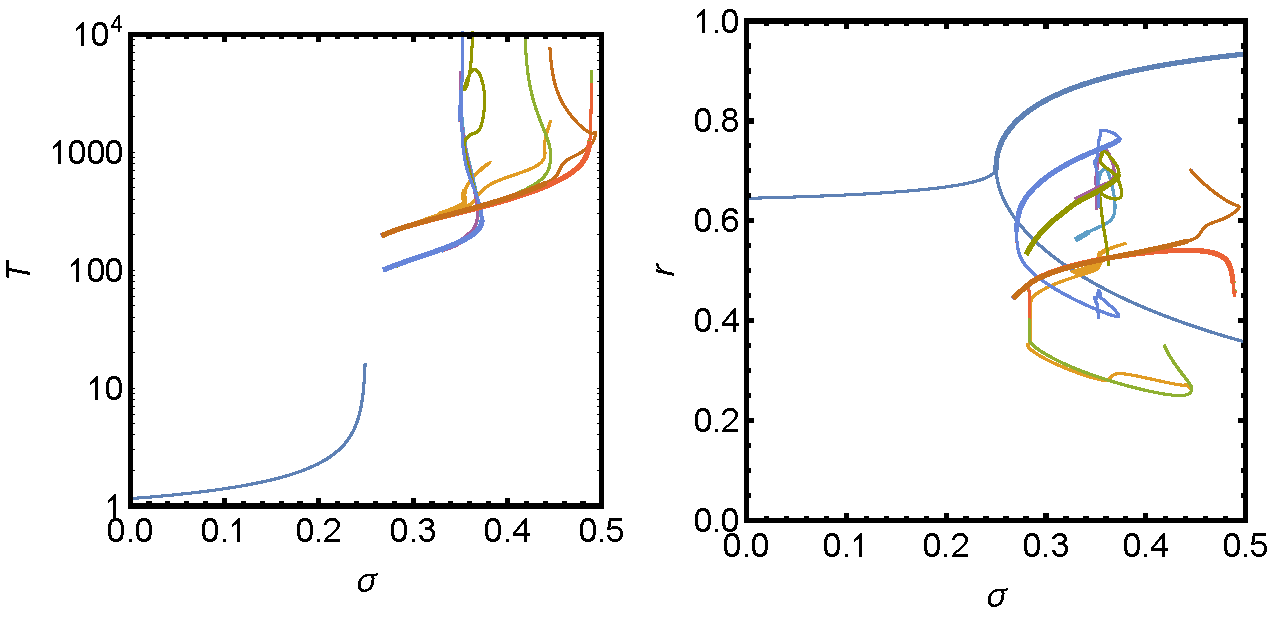
\includegraphics[width=\columnwidth]{diagram.pdf}
\caption{Bifurcation diagram with the synchronous stable branch (thick red), synchronous unstable branch (thin black), stable limit-cycle chimeras (green dots), and unstable limit-cycle chimeras (blue circles). \label{fig1}}
\end{figure}
\begin{thebibliography}{99}
\bibitem{2019_Nicolaou} Z. G. Nicolaou, D. Eroglu, and A. E. Motter. Multifaceted dynamics of Janus oscillator networks. \textit{Phys. Rev. X} \textbf{9}, 011017 (2019).
\end{thebibliography}
\end{document}
